\begin{frame}
  \frametitle{Input data}
  \begin{columns}
    \column[t]{6cm}
     \begin{table}[h!]
           \vspace*{-0.35in}
    \caption{Summary of principal data for \gls{MSBR} \cite{robertson_conceptual_1971}}
      \end{table}
    \begin{figure}[t]
      \vspace*{-0.45in}
            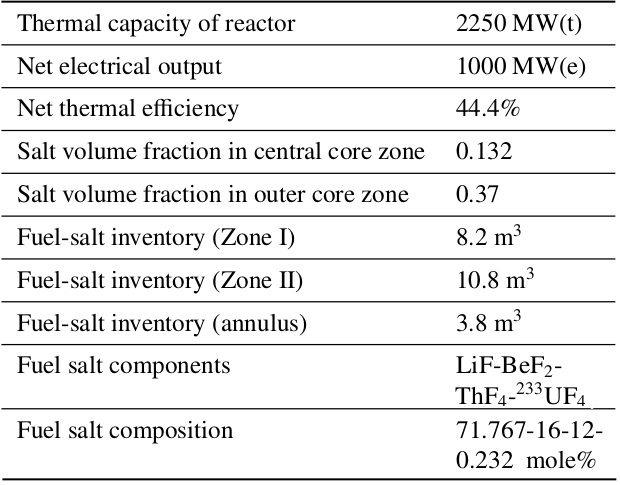
\includegraphics[height=0.87\textwidth]{./images/table_input.png}
    \end{figure}

     \column[t]{5.6cm}
           \begin{figure}
             \vspace{-0.15in}          
             \hspace*{-0.25in}
                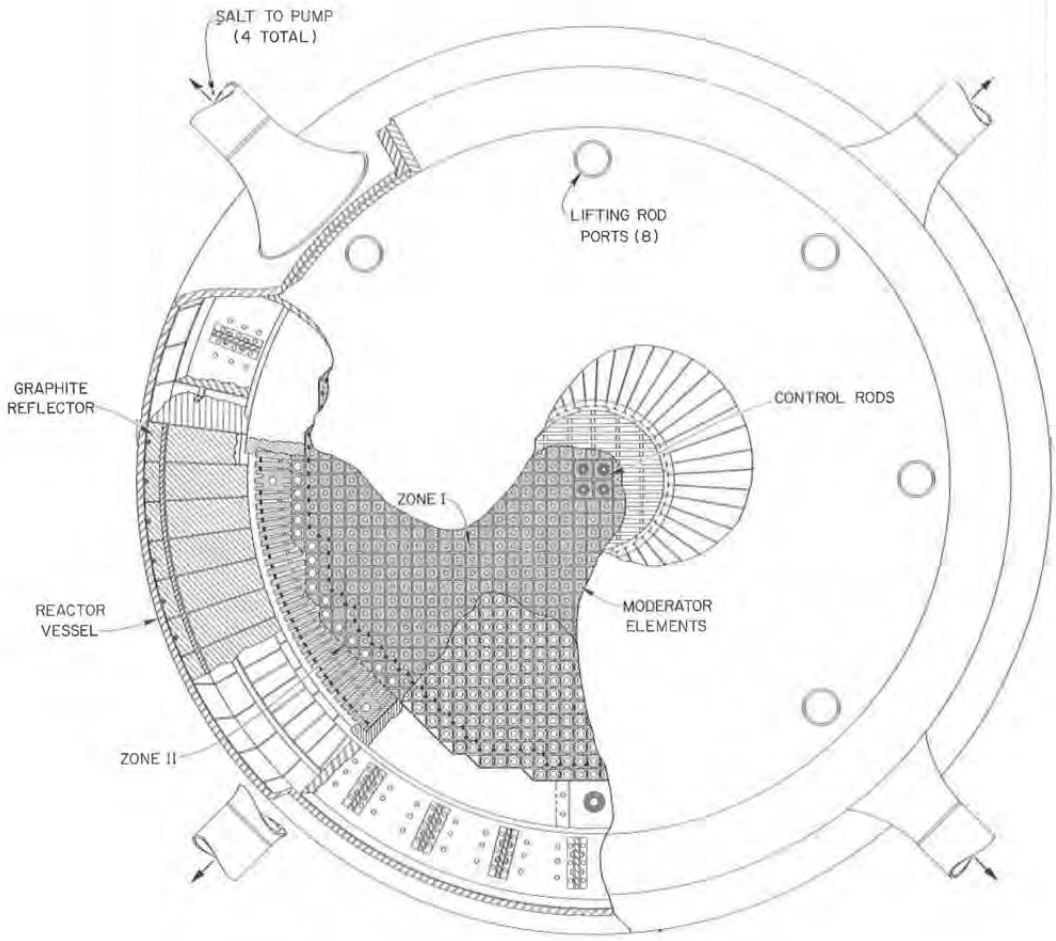
\includegraphics[height=1.03\textwidth]{./images/plan_view_vessel.png}
				\caption{Plan view of \gls{MSBR} vessel \cite{robertson_conceptual_1971}.}
      \end{figure}
  \end{columns}
              
 \end{frame}

\begin{frame}
  \frametitle{Graphite unit cell geometry}
    \begin{figure}[t]
                \vspace*{-0.2in}
                   \hspace*{-0.37in}
                \includegraphics[height=0.60\textwidth]{./images/zone_I_mesh.png}
                \vspace*{-0.05in}
                \caption{Molten Salt Breeder Reactor Zone I unit cell geometry from the reference \cite{robertson_conceptual_1971} (left) and SERPENT 2 (right).}
      \end{figure}
     
\end{frame}

\begin{frame}
\frametitle{Online reprocessing method}
	\begin{itemize}
		\item Currently, researchers typically develop custom scripts to simulate online reprocessing and refueling using stochastic (i.e. MCNP) or deterministic (i.e. SCALE) codes \cite{jeong_equilibrium_2016, powers_new_2013}.
		    \begin{figure}[t]
                \vspace*{-0.05in}
                 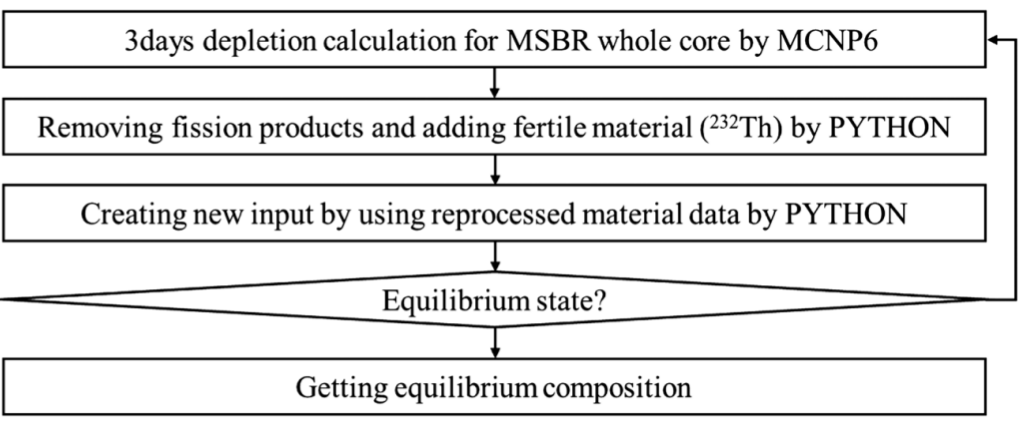
\includegraphics[height=0.30\textwidth]{./images/python_script.png}
                \vspace*{-0.05in}
                \caption{Depletion calculation principal scheme  \cite{park_whole_2015}.}
      \end{figure}
		\item SERPENT 2 allows the user to define multiple material flows into and out of the fuel and applies 								batchwise reprocessing and refueling at each step.
	\end{itemize}
\end{frame}

\begin{frame}
  \frametitle{Online reprocessing method}
     \begin{figure}[t]
                \vspace*{-0.1in}
                  % \hspace*{-0.37in}
                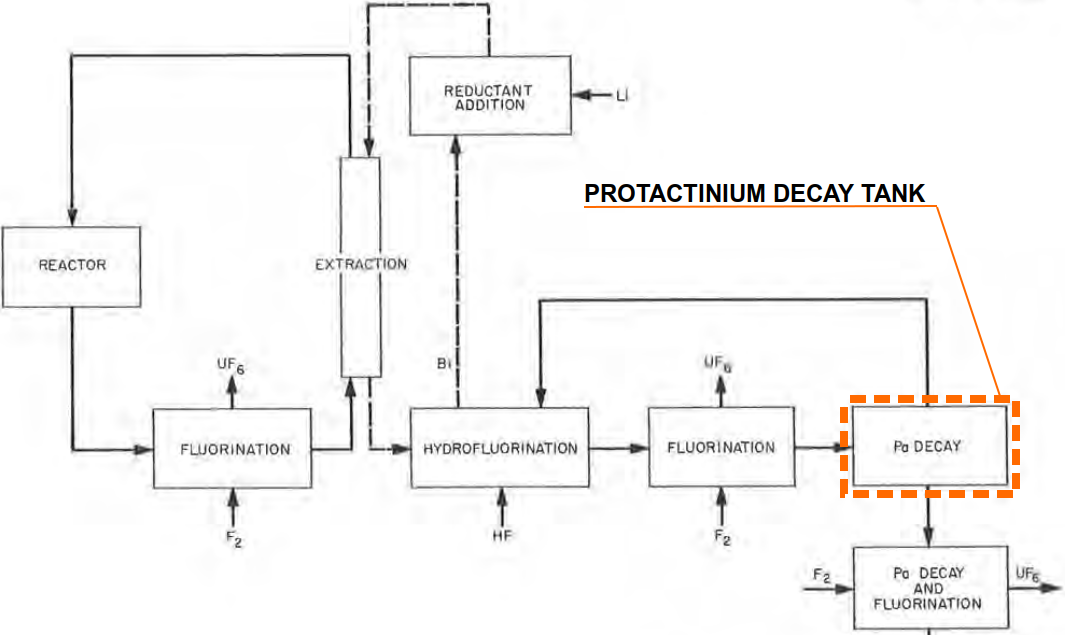
\includegraphics[height=0.45\textwidth]{./images/pa_isolation.png}
                \vspace*{-0.07in}
                \caption{Protactinium isolation with uranium removal by fluorination \cite{robertson_conceptual_1971}.}
      \end{figure}
                      \vspace*{-0.17in}
             \begin{block}{Online reprocessing approach}
               \begin{itemize}             
               \item Continuously removes all poisons, noble metals, and gases.
               \item $^{233}$Pa is continuously removed from the fuel salt into a decay tank.
               \end{itemize}
               \end{block}
               \vspace{-0.05in}
$\qquad\qquad\qquad\qquad^{232}_{90}$Th+$^1_0$n$\rightarrow^{233}_{90}$Th$\xrightarrow[\text{22.3 min}]{\beta^-}$ $^{233}_{91}$Pa$\xrightarrow[\text{26.967 d}]{\beta^-}$ $^{233}_{92}$U
\end{frame}



\begin{frame}
  \frametitle{Approximations and assumptions}
              \begin{block}{Model simplifications and assumptions}
               \begin{enumerate}
               \item Single cell model of \gls{MSBR} with periodic boundary conditions.
               \item Delayed neutron precursor drift is neglected.
               \end{enumerate}
               \end{block}

               \begin{block}{Simulation conditions and nuclear data}
               \begin{enumerate}
               \item $T_{fuel}=T_{graphite}=908$K.
               \item $\rho_{fuel}$=3.33 g/cm$^3$ and $\rho_{graphite}$=1.843 g/cm$^3$.
               \item $10^4$ neutrons per cycle for a total of 500 cycles,
                 the first 20 are inactive.
               \item ENDF/B-VII cross sections were used \cite{chadwick_endf}.
               \end{enumerate}
               \end{block}
\end{frame}

